\begin{figure}[ht]
  \centering
  \subfloat[The schematic diagram of the feature alignment module.]{%
    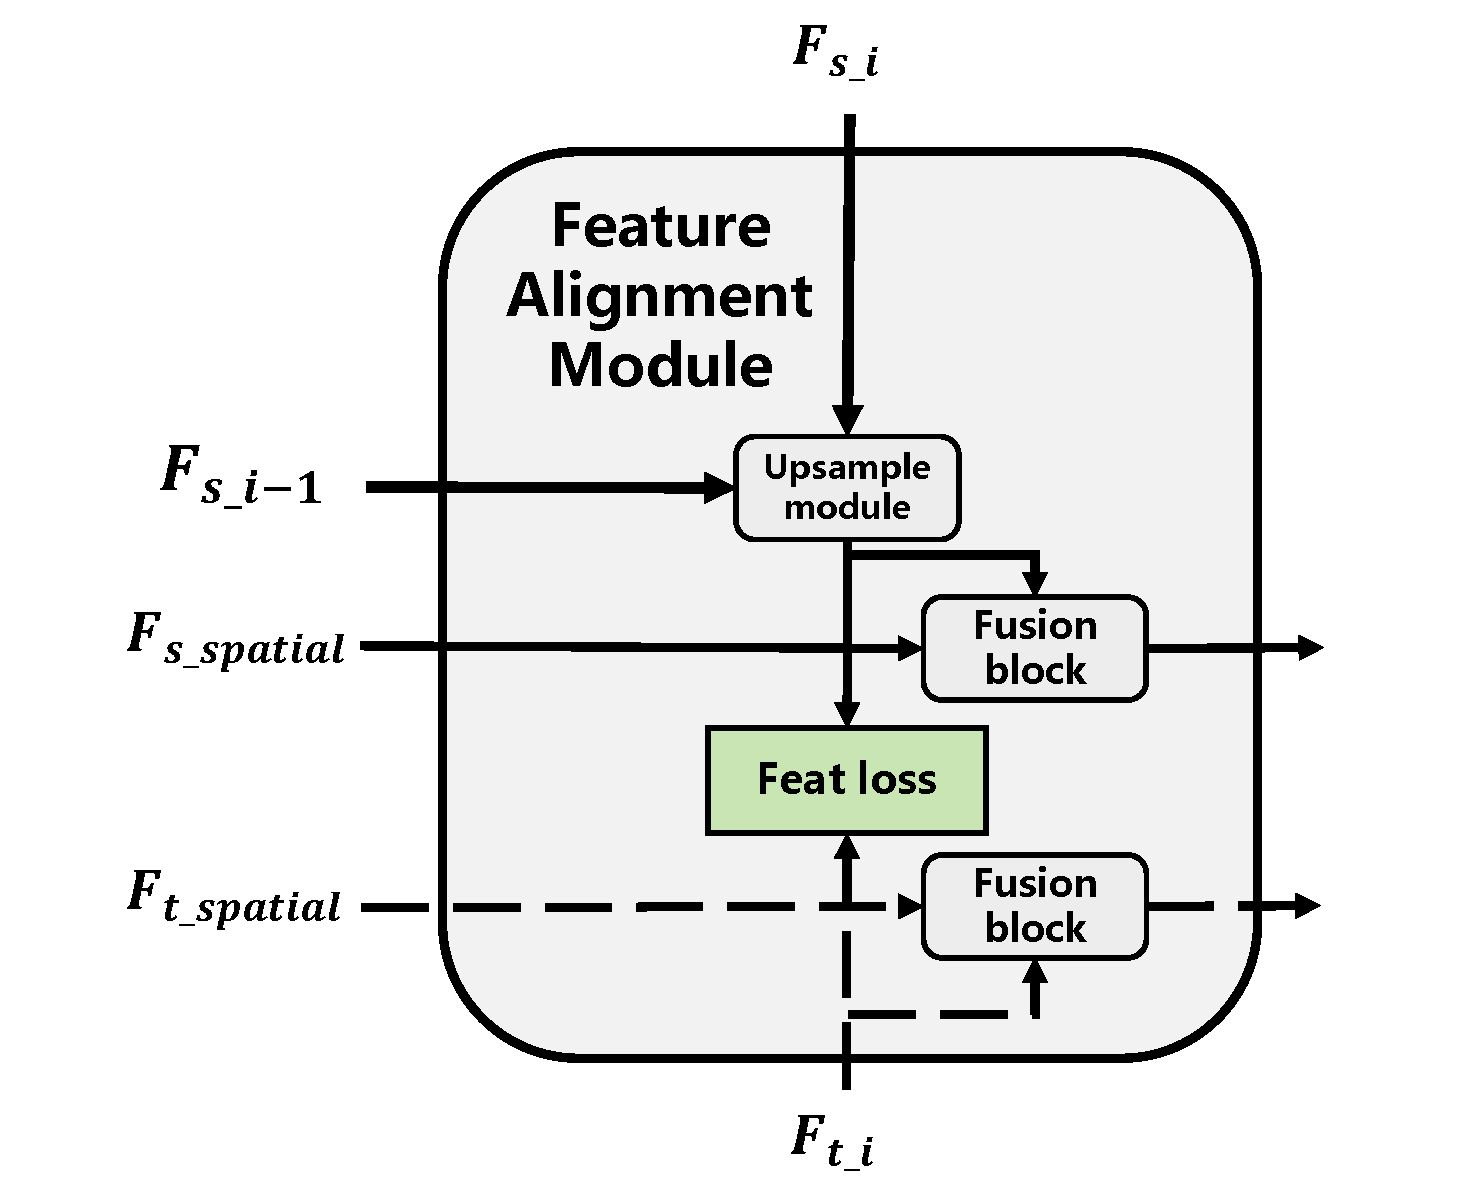
\includegraphics[width=0.45\linewidth]{feature_align_.pdf}%
    \label{fig:feat_align}%
  }
  \quad % 根据需要添加一些水平间隔
  \subfloat[The schematic diagram of the upsample module.]{%
    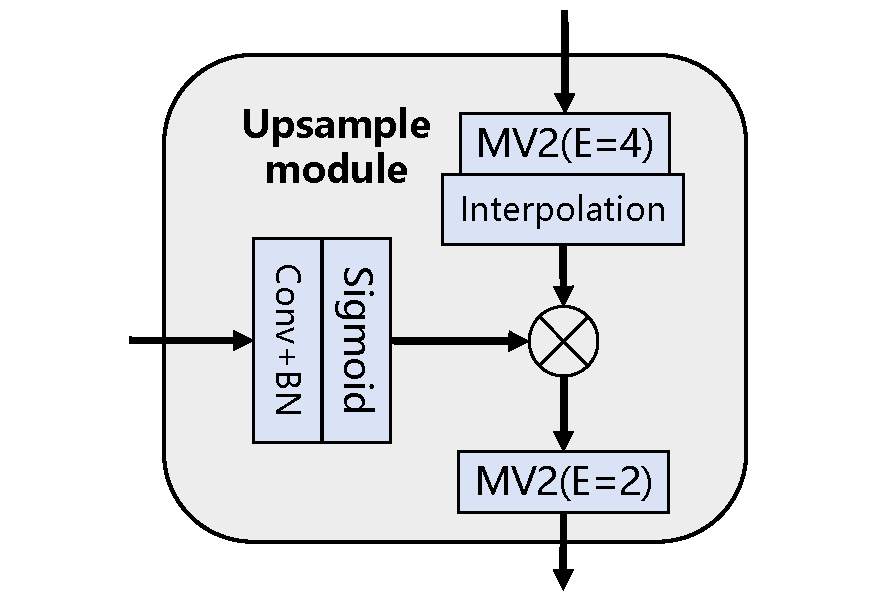
\includegraphics[width=0.45\linewidth]{upsample.pdf}%
    \label{fig:upsample}%
  }
   \caption{\textit{\textbf{Left}}: the schematic illustration of the proposed feature alignment module including an upsample module and a fusion block. \textit{$F_{s\_i}$} means feature map of student model on stage \textit{i}. \textit{$F_{t\_i}$} means feature map of teacher model on stage \textit{i}. \textit{$F_{s\_spatial}$} means feature map of student spatial branch. \textit{$F_{t\_spatial}$} means feature map of teacher spatial branch.
  \textit{\textbf{Right}} is the upsample module.}
  \label{fig:feat_align_upsample}
\end{figure}
